\documentclass[aspectratio=169]{beamer}
\usepackage{ctex}
\usepackage{graphicx}
\usepackage{amsmath}
\usepackage{booktabs}
\usepackage{hyperref}
\usepackage{pgfplots}
\usepackage{tikz}
\usetikzlibrary{positioning} % 添加此行解决"of"函数报错
\usepackage{xcolor}
\usepackage{caption}

% 定义颜色主题
\definecolor{maincolor}{RGB}{27,94,168}
\definecolor{secondcolor}{RGB}{233,131,0}

% 设置Beamer主题
\usetheme{Dresden}
\usecolortheme{whale}
\setbeamercolor{structure}{fg=maincolor}
\setbeamercolor{title}{fg=white,bg=maincolor}
\setbeamercolor{frametitle}{fg=white,bg=maincolor}
\setbeamercolor{button}{bg=secondcolor,fg=white}

% 设置字体
\setbeamerfont{frametitle}{size=\large,series=\bfseries}

% 标题页信息
\title{分布式能源系统中的储能技术}
\subtitle{锂离子电池与抽水蓄能技术的原理与应用}
\author{演讲人:周杰 \\ 2023415130128周杰~2023428020130唐玮嘉~2023428050102陈炜豪}
\institute{东莞理工学院\\化学工程与能源技术学院}
\date{\today}

\begin{document}

% 标题页
\begin{frame}
    \titlepage
\end{frame}

% 目录页
\begin{frame}
    \frametitle{目录}
    \tableofcontents
\end{frame}

% 第一部分:引言
\section{引言}
\begin{frame}
    \frametitle{研究背景}
    \begin{itemize}
        \item \textbf{能源转型背景}:全球正加速向可再生能源转型 \cite{ref1,ref3}
        \begin{itemize}
            \item 中国承诺"2030年碳达峰,2060年碳中和" \cite{ref1}
            \item 欧盟"2050年气候中和"目标 \cite{ref3}
        \end{itemize}
        \item \textbf{可再生能源挑战}:间歇性、波动性和不可预测性 \cite{ref4}
        \item \textbf{分布式能源系统}:贴近用户侧的小型发电和用能系统 \cite{ref5}
        \item \textbf{储能重要性}:平衡供需、提高系统稳定性和灵活性 \cite{ref2,ref6}
    \end{itemize}
\end{frame}

\begin{frame}
    \frametitle{分布式储能技术概述}
    \begin{columns}
        \column{0.5\textwidth}
        \textbf{分布式储能的主要价值}
        \begin{itemize}
            \item 削峰填谷
            \item 电力平衡
            \item 可再生能源消纳
            \item 提高电网稳定性
            \item 降低输配电投资
        \end{itemize}
        
        \column{0.5\textwidth}
        \textbf{主要储能技术分类}
        \begin{itemize}
            \item 电化学储能:锂离子电池、铅酸电池、流电池等
            \item 机械储能:抽水蓄能、压缩空气、飞轮等
            \item 电磁储能:超导、超级电容
            \item 热储能:相变材料、熔盐储热等
        \end{itemize}
    \end{columns}
\end{frame}

% 第二部分:锂离子电池储能
\section{锂离子电池储能技术}

\begin{frame}
    \frametitle{锂离子电池技术原理}
    \begin{columns}
        \column{0.45\textwidth}
        \textbf{工作原理}
        \begin{itemize}
            \item 基于锂离子在正负极之间的嵌入与脱嵌
            \item 充电过程:锂离子从正极脱嵌,迁移至负极并嵌入
            \item 放电过程:锂离子从负极脱嵌,迁移至正极并嵌入
        \end{itemize}
        
        \column{0.55\textwidth}
        \centering


\begin{tikzpicture}[scale=0.7, every node/.style={font=\small}]
    % 电池外壳
    \draw[ultra thick] (0,0) rectangle (8,4.8);
    
    % 电极和电解质区域
    \fill[gray!30] (0.5,0.5) rectangle (3.0,4.5);  % 负极
    \fill[blue!15] (3.0,0.5) rectangle (5.0,4.5);  % 电解质
    \fill[gray!30] (5.0,0.5) rectangle (7.5,4.5);  % 正极
    
    % 电极标记
    \node[align=center] at (1.75,2.5) {负极\\(石墨)};
    \node[align=center] at (6.25,2.5) {正极\\(金属氧化物)};
    \node[align=center, rotate=0] at (4.0,2.5) {电解质};
    
    % 充放电箭头
    \draw[->, ultra thick, red] (2.0,1.5) to[bend right=40] 
        node[midway, below, text=red] {充电} (6.0,1.5);
    \draw[<-, ultra thick, green!50!black] (2.0,3.5) to[bend right=40] 
        node[midway, above, text=green!50!black] {放电} (6.0,3.5);
    
    % 锂离子标记
    \node[red, font=\small] at (4.0,1.2) {Li$^+$};
    
    % 微观离子迁移示意(更清晰地展示锂离子移动)
    \foreach \x in {3.2,3.6,4.0,4.4,4.8}
        \draw[red,->, thick] (\x,1.5) -- ++(0,-0.15);
    \foreach \x in {3.2,3.6,4.0,4.4,4.8}
        \draw[green!50!black,->, thick] (\x,3.5) -- ++(0,0.15);
    
    % 电子流动
    \draw[->, dashed, thick, blue] (1.75,5.2) to[bend left=30] node[midway, above, text=blue] {电子流} (6.25,5.2);
    \draw[<-, dashed, thick, blue] (1.75,4.8) to[bend right=30] node[midway, below, text=blue] {} (6.25,4.8);
    
    % 图例
    \node[draw, rectangle, align=left, anchor=south west] at (0.5,-1.5) {
        \textbf{充电}: 锂离子从正极迁移到负极\\
        \textbf{放电}: 锂离子从负极迁移到正极
    };
\end{tikzpicture}

        \captionof{figure}{锂离子电池工作原理示意图}
    \end{columns}
\end{frame}


\begin{frame}
    \frametitle{锂离子电池关键参数}
    \begin{columns}
        \column{0.5\textwidth}
        \begin{itemize}
            \item \textbf{能量密度}:180-265 Wh/kg \cite{ref7}
            \item \textbf{功率密度}:250-340 W/kg \cite{ref7}
            \item \textbf{循环寿命}:1,000-10,000次 \cite{ref5}
            \item \textbf{响应时间}:毫秒级 \cite{ref4}
            \item \textbf{充放电效率}:90-95\% \cite{ref6}
            \item \textbf{自放电率}:每月约3-5\% \cite{ref7}
        \end{itemize}
        
        \column{0.5\textwidth}
        \begin{table}[h]
            \centering
            \begin{tabular}{lcc}
                \toprule
                \textbf{材料体系} & \textbf{能量密度} & \textbf{安全性} \\
                \midrule
                LFP & 中 & 高 \\
                NCM & 高 & 中 \\
                NCA & 高 & 低 \\
                LTO & 低 & 高 \\
                \bottomrule
            \end{tabular}
            \caption{主要锂电池材料体系比较}
        \end{table}
    \end{columns}
\end{frame}

\begin{frame}
    \frametitle{锂离子电池最新技术进展}
    \begin{itemize}
        \item \textbf{材料创新}
        \begin{itemize}
            \item 高镍三元材料(NCM811, NCA91.5):能量密度提升至300Wh/kg以上
            \item 硅碳负极:提高负极容量,理论容量可达4200mAh/g
            \item 固态电解质:提高安全性,实现能量密度500Wh/kg以上
        \end{itemize}
        \item \textbf{电池管理系统(BMS)进步}
        \begin{itemize}
            \item 基于大数据和人工智能的健康状态(SOH)预测:准确率提升20\%以上
            \item 云端基于数字孪生的电池远程运维平台
        \end{itemize}
        \item \textbf{模组集成技术}
        \begin{itemize}
            \item 无模组设计(CTP/CTC):体积能量密度提升15-20\%
            \item 液冷技术:充放电速率提高,散热效率提升40\%
        \end{itemize}
    \end{itemize}
\end{frame}

\begin{frame}
    \frametitle{锂离子电池储能系统架构}
    \begin{figure}[ht]
    \centering
        \begin{tikzpicture}[node distance=1.0cm, auto, scale=0.6, transform shape] % 缩小节点间距和整体比例
            % 电池单元
            \node[draw, rectangle, minimum width=1.2cm, minimum height=0.8cm, fill=gray!20] (cell) {电池单元};
            
            % 电池模组
            \node[draw, rectangle, minimum width=2cm, minimum height=1.2cm, fill=gray!30, below=of cell] (module) {电池模组};
            \draw[->] (cell) -- (module);
            
            % 电池包
            \node[draw, rectangle, minimum width=3cm, minimum height=1.6cm, fill=gray!40, below=of module] (pack) {电池包/机柜};
            \draw[->] (module) -- (pack);
            
            % BMS
            \node[draw, rectangle, minimum width=1.8cm, minimum height=0.8cm, fill=blue!20, right=of module] (bms) {BMS};
            \draw[<->] (module) -- (bms);
            \draw[<->] (pack) -- (bms);
            
            % PCS
            \node[draw, rectangle, minimum width=2cm, minimum height=1.2cm, fill=green!20, below=of pack] (pcs) {PCS};
            \draw[<->] (pack) -- (pcs);
            
            % EMS
            \node[draw, rectangle, minimum width=2.5cm, minimum height=1.2cm, fill=orange!20, right=of pack] (ems) {EMS};
            \draw[<->] (bms) -- (ems);
            \draw[<->] (pcs) -- (ems);
            
            % 电网/负载
            \node[draw, rectangle, minimum width=2.5cm, minimum height=0.8cm, fill=yellow!20, below=of pcs] (grid) {电网/负载};
            \draw[<->] (pcs) -- (grid);
        \end{tikzpicture}
    \caption{锂离子电池储能系统架构图}
    \end{figure}

\end{frame}

\begin{frame}
    \frametitle{国内案例:国网青海海南州共和光储系统}
    \begin{columns}
        \column{0.6\textwidth}
        \textbf{项目概况}
        \begin{itemize}
            \item \textbf{地点}:青海省海南藏族自治州共和县
            \item \textbf{规模}:100MW/100MWh锂电池储能系统
            \item \textbf{配套}:光伏装机500MW
            \item \textbf{建成时间}:2021年12月并网
            \item \textbf{系统供应商}:宁德时代(CATL)
        \end{itemize}
        
        \textbf{技术特点}
        \begin{itemize}
            \item 采用磷酸铁锂电池技术
            \item 应用液冷技术,适应高原地区温差大环境
            \item 集装箱一体化设计,快速部署
        \end{itemize}
        
        \column{0.4\textwidth}
        \centering
        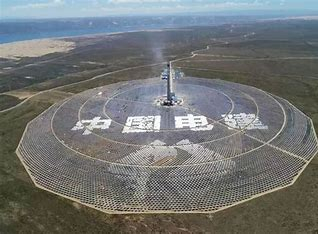
\includegraphics[width=\textwidth]{fig/青海共和光储项目示意图.jpg}
        \captionof{figure}{青海共和光储项目示意图}
    \end{columns}
\end{frame}

\begin{frame}
    \frametitle{国内案例:国网青海海南州共和光储系统(续)}
    \begin{itemize}
        \item \textbf{应用场景}
        \begin{itemize}
            \item 可再生能源消纳:平抑光伏出力波动
            \item 电网调峰:日间储存过剩光伏电力,夜间释放
            \item 一次调频:响应电网频率波动,提供快速响应服务
            \item 黑启动:区域电网故障时提供恢复电源
        \end{itemize}
        
        \item \textbf{项目效益}
        \begin{itemize}
            \item 提高光伏消纳率约10\%
            \item 减少弃光约2000万kWh/年
            \item 降低电网波动率87\%以上
            \item 减少碳排放约1.6万吨/年
            \item 延缓新建输电线路投资
        \end{itemize}
    \end{itemize}
\end{frame}

\begin{frame}
    \frametitle{国外案例:澳大利亚Hornsdale电池储能电站}
    \begin{columns}
        \column{0.55\textwidth}
        \textbf{项目概况}
        \begin{itemize}
            \item \textbf{地点}:澳大利亚南澳大利亚州
            \item \textbf{规模}:150MW/194MWh
            \item \textbf{建成时间}:2017年首期,2020年扩建
            \item \textbf{供应商}:特斯拉Megapack
        \end{itemize}
        
        \textbf{背景}:2016年南澳大利亚州发生严重停电事件后建设
        
        \column{0.45\textwidth}
        \centering
        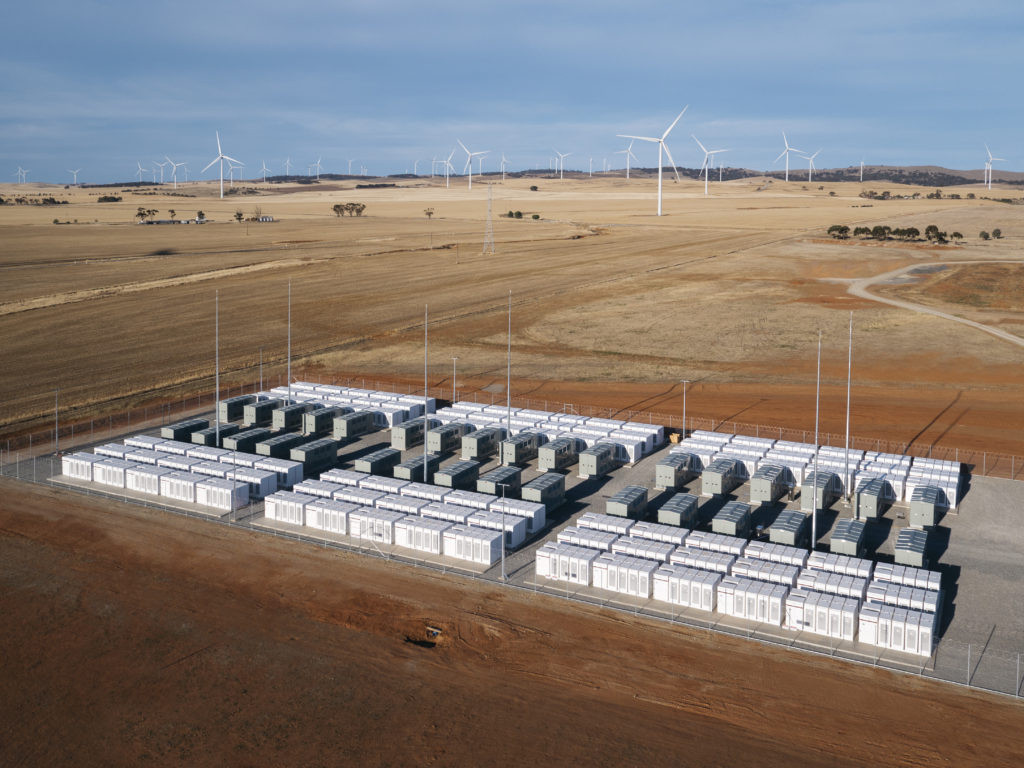
\includegraphics[width=\textwidth]{fig/Hornsdale电池储能电站.jpg}
        \captionof{figure}{Hornsdale电池储能电站}
    \end{columns}
\end{frame}

\begin{frame}
    \frametitle{国外案例:澳大利亚Hornsdale电池储能电站(续)}
    \begin{itemize}
        \item \textbf{系统性能}
        \begin{itemize}
            \item 响应时间:140毫秒(远低于传统电源的秒级响应)
            \item 调频精度:优于传统煤电机组10倍以上
        \end{itemize}
        
        \item \textbf{应用场景}
        \begin{itemize}
            \item 电网频率控制服务(FCAS)
            \item 虚拟输电线路服务
            \item 电力批发市场套利
            \item 系统惯量服务
        \end{itemize}
        
        \item \textbf{项目效益}
        \begin{itemize}
            \item 节省电网服务成本超过1.5亿澳元(2017-2020)
            \item 电网频率合格率提升30\%以上
            \item 减少碳排放约50万吨/年
            \item 投资回报周期:4-5年
        \end{itemize}
    \end{itemize}
\end{frame}

% 第三部分:抽水蓄能
\section{抽水蓄能技术}

\begin{frame}
    \frametitle{抽水蓄能技术原理}
    \begin{columns}
        \column{0.5\textwidth}
        \textbf{工作原理}
        \begin{itemize}
            \item 基于势能储存与转换
            \item 低谷电力:抽水至高水库储存势能
            \item 高峰时段:放水发电转换为电能
            \item 能量存储公式:
            \begin{equation}
                E = \eta \cdot \rho \cdot g \cdot h \cdot V
            \end{equation}
            其中:$\eta$为效率,$\rho$为水密度,$g$为重力加速度,$h$为水头高度,$V$为水量
        \end{itemize}
        
        \column{0.5\textwidth}
        \centering
        \begin{tikzpicture}[scale=0.6]
            % 上水库
            \draw[thick] (0,4) ellipse (2 and 0.5);
            \draw[thick] (-2,4) -- (-2,3);
            \draw[thick] (2,4) -- (2,3);
            \fill[blue!30] (-2,3) arc (180:360:2 and 0.5) -- (2,4) arc (0:180:2 and 0.5) -- cycle;
            \node at (0,4) {上水库};
            
            % 下水库
            \draw[thick] (0,0) ellipse (3 and 0.7);
            \draw[thick] (-3,0) -- (-3,-1);
            \draw[thick] (3,0) -- (3,-1);
            \fill[blue!30] (-3,-1) arc (180:360:3 and 0.7) -- (3,0) arc (0:180:3 and 0.7) -- cycle;
            \node at (0,-0.5) {下水库};
            
            % 水管
            \draw[thick] (-1,3) -- (-2,0.5);
            
            % 发电机组
            \filldraw[fill=gray!40] (-2.5,1.5) rectangle (-1.5,2.5);
            \node at (-2,2) {泵/机组};
            
            % 箭头标识
            \draw[->, thick, red] (-1.8,3) -- (-1.8,2.6) node[right] {放水发电};
            \draw[->, thick, green] (-1.8,1.4) -- (-1.8,1) node[right] {抽水蓄能};
        \end{tikzpicture}
        \captionof{figure}{抽水蓄能系统示意图}
    \end{columns}
\end{frame}

\begin{frame}
    \frametitle{抽水蓄能关键参数}
    \begin{columns}
        \column{0.5\textwidth}
        \begin{itemize}
            \item \textbf{能量密度}:低,约0.5-1.5 Wh/kg
            \item \textbf{效率}:70-85\%(往返效率)
            \item \textbf{响应时间}:分钟级(传统),秒级(新型)
            \item \textbf{寿命}:40-60年
            \item \textbf{自放电率}:极低(主要是蒸发损失)
            \item \textbf{规模}:大型,通常100MW-3000MW
        \end{itemize}
        
        \column{0.5\textwidth}
        \begin{table}[h]
            \centering
            \begin{tabular}{lcc}
                \toprule
                \textbf{类型} & \textbf{优点} & \textbf{缺点} \\
                \midrule
                常规 & 成熟可靠 & 选址受限 \\
                海水 & 容量大 & 腐蚀严重 \\
                地下 & 占地少 & 建设成本高 \\
                小型化 & 灵活分散 & 经济性差 \\
                \bottomrule
            \end{tabular}
            \caption{抽水蓄能电站类型对比}
        \end{table}
    \end{columns}
\end{frame}

\begin{frame}
    \frametitle{抽水蓄能最新技术进展}
    \begin{itemize}
        \item \textbf{可变速抽水蓄能技术}
        \begin{itemize}
            \item 采用双馈异步电机或全转换器同步电机
            \item 优势:发电模式下可调节50-100\%额定功率
            \item 效益:提高电网调频能力,往返效率提升3-5\%
        \end{itemize}
        
        \item \textbf{小型模块化抽水蓄能}
        \begin{itemize}
            \item 单机容量:1-20MW
            \item 设计特点:标准化设计,工厂预制装配
            \item 应用:分布式能源系统、微电网
        \end{itemize}
        
        \item \textbf{泵蓄与风光互补系统集成技术}
        \begin{itemize}
            \item 风光泵储一体化设计
            \item 联合优化调度算法:效率提升10-15\%
            \item 虚拟同步机技术:提供系统惯量与短路容量
        \end{itemize}
    \end{itemize}
\end{frame}

\begin{frame}
    \frametitle{国内案例:广东惠州抽水蓄能电站}
    \begin{columns}
        \column{0.6\textwidth}
        \textbf{项目概况}
        \begin{itemize}
            \item \textbf{地点}:广东省惠州市龙门县
            \item \textbf{装机规模}:2400MW(8×300MW)
            \item \textbf{蓄能能力}:约16.8GWh
            \item \textbf{投产时间}:2011年全部投产
            \item \textbf{静态投资}:约120亿元人民币
        \end{itemize}
        
        \textbf{技术特点}
        \begin{itemize}
            \item 采用单级混流可逆式水泵水轮机
            \item 上下水库有效落差:507米
            \item 首次采用全地下式厂房布置
        \end{itemize}
        
        \column{0.4\textwidth}
        \centering
        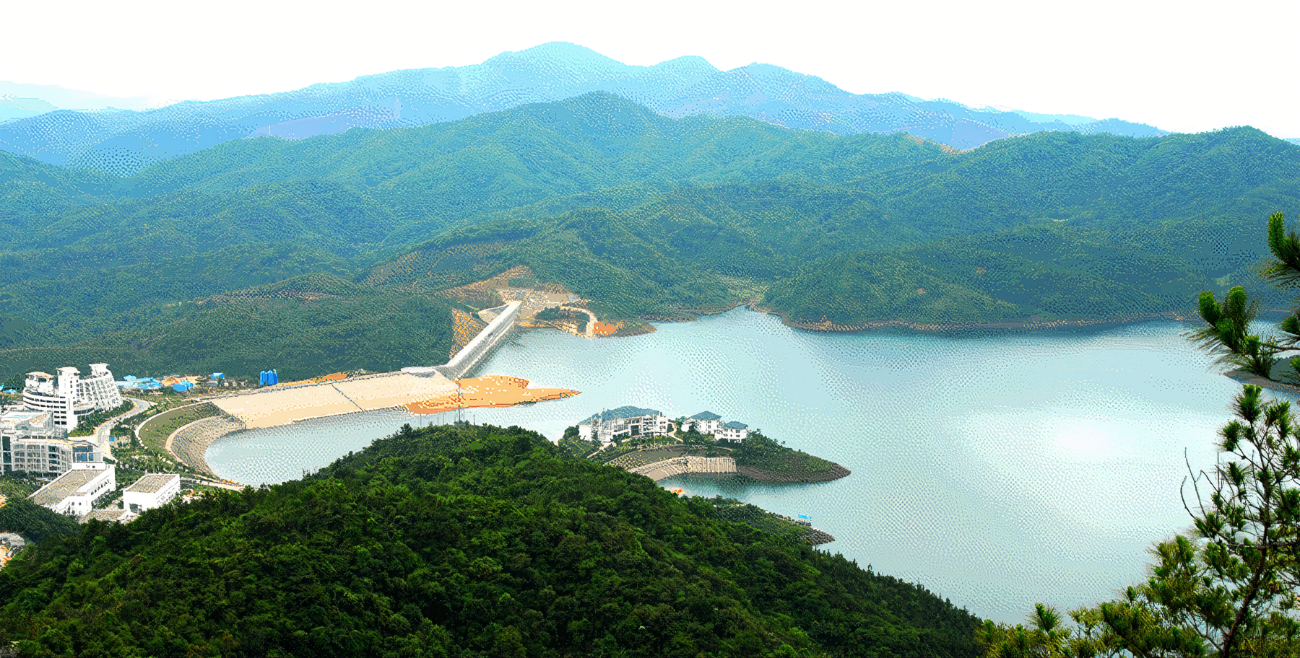
\includegraphics[width=\textwidth]{fig/惠州抽水蓄能电站示意图.jpg}
        \captionof{figure}{惠州抽水蓄能电站示意图}
    \end{columns}
\end{frame}

\begin{frame}
    \frametitle{国内案例:广东惠州抽水蓄能电站(续)}
    \begin{itemize}
        \item \textbf{运行模式}
        \begin{itemize}
            \item 电网调峰:夜间低谷抽水,白天高峰发电
            \item 系统备用:提供旋转备用、黑启动能力
            \item 频率调节:响应电网频率波动,提供调频服务
        \end{itemize}
        
        \item \textbf{项目效益}
        \begin{itemize}
            \item 增加广东电网调峰能力达2400MW
            \item 减少火电机组深度调峰损耗,每年节约标煤约37万吨
            \item 提高电网安全运行水平,降低系统备用容量
            \item 支持广东核电、风电发展,促进低碳能源结构转型
            \item 减少二氧化碳排放约100万吨/年
        \end{itemize}
    \end{itemize}
\end{frame}

\begin{frame}
    \frametitle{国外案例:瑞士Nant de Drance抽水蓄能电站}
    \begin{columns}
        \column{0.55\textwidth}
        \textbf{项目概况}
        \begin{itemize}
            \item \textbf{地点}:瑞士瓦莱州阿尔卑斯山区
            \item \textbf{装机规模}:900MW(6×150MW)
            \item \textbf{蓄能能力}:约20GWh
            \item \textbf{投产时间}:2022年全面投入商业运营
            \item \textbf{投资额}:约19亿瑞士法郎
        \end{itemize}
        
        \column{0.45\textwidth}
        \centering
        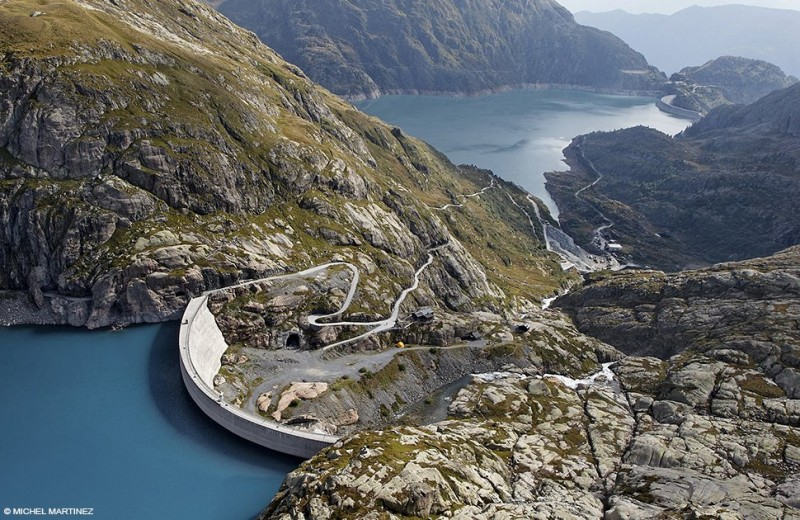
\includegraphics[width=\textwidth]{fig/Nant de Drance电站.jpg}
        \captionof{figure}{Nant de Drance电站}
    \end{columns}
\end{frame}

\begin{frame}
    \frametitle{国外案例:瑞士Nant de Drance抽水蓄能电站(续)}
    \begin{itemize}
        \item \textbf{技术特点}
        \begin{itemize}
            \item 采用最新可变速技术,响应时间小于10秒
            \item 380米落差,欧洲最高水头抽水蓄能电站之一
            \item 全地下洞室系统,环境影响小
            \item 机组额定功率:150MW,效率高达80\%以上
        \end{itemize}
        
        \item \textbf{项目效益}
        \begin{itemize}
            \item 为瑞士和欧洲电网提供调峰、调频服务
            \item 促进欧洲可再生能源并网(特别是北海风电)
            \item 跨国电力交易平台(连接法国、德国、意大利电网)
            \item 减少碳排放约40万吨/年
            \item 提高区域电力系统稳定性和可靠性
        \end{itemize}
    \end{itemize}
\end{frame}

% 第四部分:储能技术对比与展望
\section{储能技术对比与展望}

\begin{frame}
    \frametitle{储能技术比较}
    \begin{table}
        \centering
        \begin{tabular}{lcc}
            \toprule
            \textbf{参数} & \textbf{锂离子电池} & \textbf{抽水蓄能} \\
            \midrule
            能量密度 & 高 (180-265 Wh/kg) & 低 (0.5-1.5 Wh/kg) \\
            响应速度 & 毫秒级 & 秒-分钟级 \\
            循环寿命 & 1,000-10,000次 & 40-60年 \\
            效率 & 90-95\% & 70-85\% \\
            适用规模 & kW-100MW级 & 10MW-3GW级 \\
            地理限制 & 低 & 高 \\
            投资成本 & 1500-3000元/kWh & 3000-8000元/kW \\
            运维成本 & 中等 & 低 \\
            \bottomrule
        \end{tabular}
        \caption{锂离子电池与抽水蓄能技术对比}
    \end{table}
\end{frame}

\begin{frame}
    \frametitle{分布式储能应用场景比较}
    \begin{columns}
        \column{0.5\textwidth}
        \textbf{锂离子电池优势场景}
        \begin{itemize}
            \item 分布式光伏配套储能
            \item 商业楼宇需量响应
            \item 微电网稳定控制
            \item 电动汽车充电站辅助
            \item 家庭能源管理系统
            \item 电网辅助服务(调频)
        \end{itemize}
        
        \column{0.5\textwidth}
        \textbf{抽水蓄能优势场景}
        \begin{itemize}
            \item 大型可再生能源基地配套
            \item 区域电网调峰调频
            \item 电网黑启动支撑
            \item 输电通道阻塞管理
            \item 系统惯量与短路容量支撑
            \item 跨区域负荷转移
        \end{itemize}
    \end{columns}
\end{frame}

\begin{frame}
    \frametitle{储能技术发展趋势}
    \begin{itemize}
        \item \textbf{技术协同}
        \begin{itemize}
            \item 多种储能技术互补:快响应+长时间+大容量
            \item 储能与能源转换技术融合(如Power-to-Gas)
        \end{itemize}
        
        \item \textbf{商业模式创新}
        \begin{itemize}
            \item 共享储能平台
            \item 储能即服务(SEaaS)
            \item 虚拟电厂聚合交易
        \end{itemize}
        
        \item \textbf{技术发展方向}
        \begin{itemize}
            \item 锂电池:固态电池、钠离子电池、锂硫电池
            \item 抽水蓄能:小型化、模块化、智能化
            \item 系统集成:多能互补、源网荷储一体化
        \end{itemize}
        
        \item \textbf{政策支持}
        \begin{itemize}
            \item 国家层面:能源"十四五"规划、新型电力系统
            \item 地方层面:储能配置要求、峰谷电价机制
            \item 市场机制:电力辅助服务市场、容量电价
        \end{itemize}
    \end{itemize}
\end{frame}

\begin{frame}
    \frametitle{我国储能发展规划与目标}
    \begin{itemize}
        \item \textbf{《新型储能发展实施方案(2021-2025年)》} \cite{ref1}
        \begin{itemize}
            \item 2025年:新型储能装机规模达30GW以上
            \item 锂电池成本降低30\%以上
            \item 建立健全储能市场机制
        \end{itemize}
        
        \item \textbf{《"十四五"可再生能源发展规划》} \cite{ref2}
        \begin{itemize}
            \item 风电、光伏新增项目配置20\%以上储能容量
            \item 抽水蓄能2025年装机目标62GW \cite{ref8}
            \item 支持"新能源+储能"示范项目建设
        \end{itemize}
        
        \item \textbf{《电力发展"十四五"规划》}
        \begin{itemize}
            \item 构建新型电力系统,储能为关键支撑
            \item 促进源网荷储协调发展
            \item 加快储能技术创新与产业化
        \end{itemize}
    \end{itemize}
\end{frame}

% 第五部分:结论
\section{结论}

\begin{frame}
    \frametitle{总结与建议}
    \begin{columns}
        \column{0.5\textwidth}
        \textbf{结论}
        \begin{itemize}
            \item 储能是分布式能源系统必要组成部分
            \item 锂电池适合短时、分散、灵活应用场景
            \item 抽水蓄能适合大规模、长时间调节场景
            \item 技术进步降低储能成本,提高系统效能
            \item 储能项目经济性日益提升
        \end{itemize}
        
        \column{0.5\textwidth}
        \textbf{建议}
        \begin{itemize}
            \item 加强储能关键技术研发投入
            \item 完善电力市场机制设计,体现储能价值
            \item 因地制宜选择合适储能技术路线
            \item 鼓励多样化商业模式创新
            \item 储能与能源互联网协同发展
        \end{itemize}
    \end{columns}
\end{frame}

\begin{frame}
    \frametitle{参考文献}
    \scriptsize  % 缩小字体(可选值:\tiny, \scriptsize, \footnotesize, \small)
    \setlength{\itemsep}{-0.2em} % 减小条目间距
    \begin{thebibliography}{99}
        \bibitem{ref1} 国家发改委, 国家能源局. 《新型储能发展实施方案(2021-2025年)》[Z]. 2021.
        \bibitem{ref2} 中国电力企业联合会. 《中国电力行业年度发展报告2023》[R]. 2023.
        \bibitem{ref3} International Energy Agency (IEA). Energy Storage Report 2024 [R]. 2024.
        \bibitem{ref4} P. Denholm, et al. The Value of Energy Storage for Grid Applications [J]. National Renewable Energy Laboratory, 2023.
        \bibitem{ref5} 国网能源研究院. 《中国储能产业发展白皮书》[R]. 2024.
        \bibitem{ref6} 阮洪兵, 邵志刚, 等. 大规模可再生能源并网中储能关键技术研究进展[J]. 中国电机工程学报, 2023, 43(5): 1498-1509.
        \bibitem{ref7} BloombergNEF. 2024 Battery Price Survey [R]. 2024.
        \bibitem{ref8} International Hydropower Association. Pumped Storage Tracking Tool [DB/OL]. 2024.
    \end{thebibliography}
    \vspace{-1em}
    \bibliographystyle{IEEEtran}
    \bibliography{IEEEexample}
\end{frame}

\begin{frame}
    \frametitle{谢谢}
    \centering
    \LARGE \textbf{谢谢观看}\\
    \vspace{1cm}
    \Large 欢迎提问
\end{frame}



\end{document}